\chapter{Statistical Tests}

\section{Hypothesis tests}\label{sec:hypotheses} \index{general}{hypotheses}

A statistical hypothesis test is a method of statistical inference using data from a scientific study. In statistics, a result is called \emph{statistically significant} if it has been predicted as unlikely to have occurred by chance alone, according to a pre-determined threshold probability, the \emph{significance level}. These tests are used in determining what outcomes of a study would lead to a rejection of the \emph{null hypothesis} for a pre-specified \emph{level of significance}. The critical region of a hypothesis test is the set of all outcomes which cause the null hypothesis to be rejected in favor of the \emph{alternative hypothesis}.

A typical approach is as follows: you

\begin{itemize}
  \item   state your hypothesis.
  \item   decide which value you want to test your hypothesis on, which is called the \emph{test statistic T}.
  \item   compute from the observations the observed value $t_{obs}$ of the test statistic.
  \item   Calculate the \emph{p-value}. This is the probability, under the null hypothesis, of sampling a test statistic at least as extreme as that which was observed.
  \item   Reject the null hypothesis, in favor of the alternative hypothesis, if and only if the p-value is less than the significance level (the selected probability) threshold. If $p<0.05$, the difference between your sample and the value that you check is \emph{significant}. If $p<0.001$, we speak of a \emph{highly significant} difference.
\end{itemize}

Keep in mind that unlikely events \emph{do} happen: In 1980, for example, a woman named Maureen Wilcox played the Rhode Island and the Massachusetts lotteries at the same time. And she hit the correct numbers for both. Unfortunately, she picked all the correct numbers for Massachusetts on her Rhode Island ticket, and all the right Rhode Island numbers on her Massachusetts ticket. Such events are unlikely - but they do happen!


\textbf{Example 1: } Let us compare the weight of two groups of subject. Then the \emph{null hypothesis} is that there is \emph{null} difference in the weight between the two groups. If a statistical comparison of the weight produces a p-value of 0.03, this means that \emph{the probability that the null hypothesis is correct is 0.03, or 3\%}. Since this probability is quite low, we say that \emph{there is a significant difference between the weight of the two groups}.

\textbf{Example 2: } If we want to check the assumption that the mean value of a group is 7, then the null hypothesis would be: \emph{"We assume that there is null difference between the mean value in our poulation and the value 7."}

\subsection{Types of Error}
In hypothesis testing, two types of errors can occur:

\subsubsection{Type I errors} \index{general}{error!Type I} \index{general}{power}
These are errors, where you get a significant result despite the fact that the hypothesis is true. The likelihood of a Type I error is commonly indicated with $\alpha$, and \emph{is set before you start the data analysis}. In quality control, a Type I error is called \emph{producer risk}, because you keep a produced item despite the fact that it meets the regulatory requirements.

For example, assume that the population of young Austrian adults has a mean IQ of 105 (i.e. we are smarter than the rest) and a standard deviation of 15. We now want to check if the average FH student in Linz has the same IQ as the average Austrian, and we select 20 students. We set $\alpha=0.05$, i.e. we set our significance level to 95\%.
Let us now assume that the average student has in fact the same IQ as the average Austrian. If we repeat our study 20 times, we will find one of those 20 times that our sample mean is significantly different from the Austrian average IQ. Such a finding would be a false result, despite the fact that our assumption is correct, and would constitute a \emph{type I error}.

\subsubsection{Type II errors and Test Power}\index{general}{error!Type II}
If we want to answer the question "How much chance do we have to reject the null hypothesis when the alternative is in fact true?" Or in other words, "What’s the probability of detecting a real effect?" we are faced with a different problem. To answer these questions, we need an \emph{alternative hypothesis}.

For the example given above, an \emph{alternative hypothesis} could be: "We assume that our population has a mean value of 6."

A \emph{Type II error} is an error, where you do \emph{not} get a significant result, despite the fact that the null-hypothesis is false.  In quality control, a Type II error is called a \emph{consumer risk}, because the consumer obtains an item that does not meet the regulatory requirements.

The probability for this type of error is commonly indicated with $\beta$. The \emph{power} of a statistical test is defined as $(1-\beta)*100$, and is the chance of correctly accepting the alternate hypothesis. Figure \ref{fig:power1} shows the meaning of the \emph{power} of a statistical test. Note that for finding the power of a test, you need an alternative hypothesis.

\subsection{Sample Size}\index{general}{sample size}
The power of a statistical test depends on four factors:

\begin{enumerate}
  \item  $\alpha$, the probability for Type I errors
  \item  $\beta$, the probability for Type II errors ( $\Rightarrow$ power of the test)
  \item  $d$, the \emph{effect size}, i.e. the magnitude of the investigated effect relative to $\sigma$, the standard deviation of the sample
  \item  $n$, the sample size
\end{enumerate}

Only 3 of these 4 parameters can be chosen, the $4^{th}$ is then automatically fixed.

The absolute size of the difference $D$ between mean treatment outcomes that will answer the clinical question being posed is often called \emph{clinical significance} or \emph{clinical relevance}.

\begin{figure}[!ht]
  \centering
  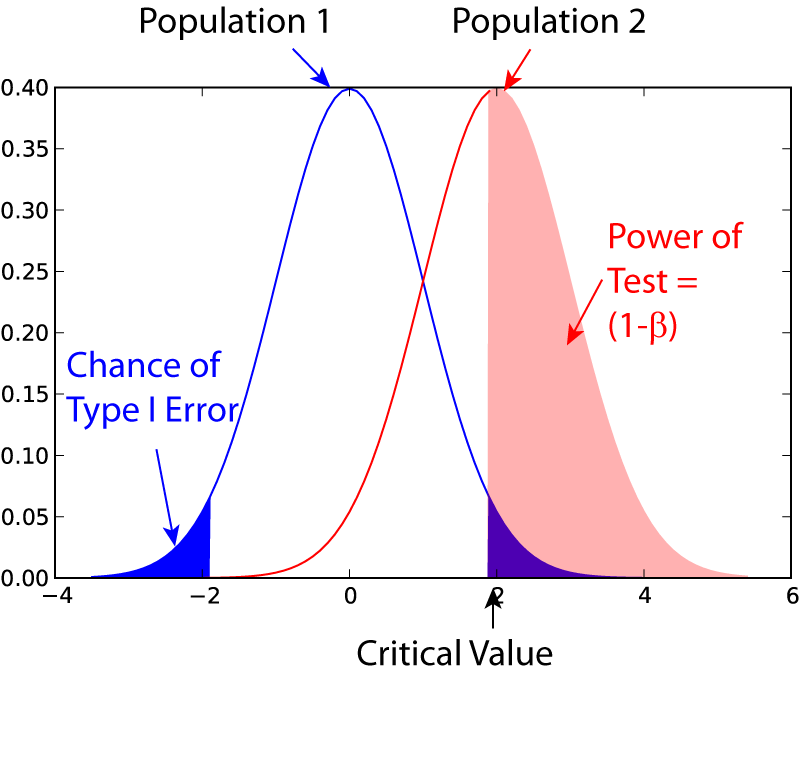
\includegraphics[width=0.5\textwidth]{../Images/power1.png}\\
  \caption{\emph{Power} of a statistical test, for comparing the mean value of two given distributions.}\label{fig:power1}
\end{figure}

\begin{figure}[!ht]
  \centering
  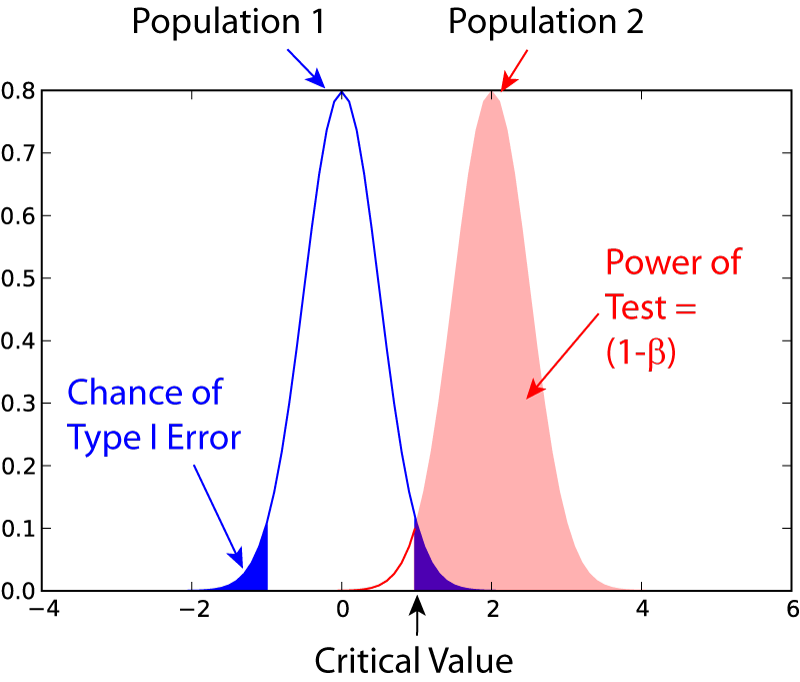
\includegraphics[width=0.5\textwidth]{../Images/power2.png}\\
  \caption{Effect of an increase in sampling size on the power of a test.}\label{fig:power2}
\end{figure}

\subsubsection{Examples for some special cases}

For a test on one mean, this leads to a \emph{minimum sample number} of

\begin{equation}
  n = \frac{{({z_{1 - \alpha /2}} + {z_{1 - \beta }})}^2}{d^2}
\end{equation}

Here z is the standardized normal variable (see also chapter \ref{sec:normalDistribution})

\begin{equation}
  z = \frac{x-\mu}{\sigma} .
\end{equation}

and $d = \frac{D}{\sigma}$ the effect size.

For finding a difference between two normally distributed means, the minimum number of samples we need in each group to detect an absolute difference $D$ is

\begin{equation}
  {n_1} = {n_2} = \frac{{({z_{1 - \alpha /2}} + {z_{1 - \beta }})}^2(\sigma _1^2 + \sigma _2^2)}{D^2} .
\end{equation}

\subsubsection{Programs: SampleSize}

\PyImg "sampleSize.py" (p \pageref{py:sampleSize}): sample size calculation for normally distributed groups.
\index{python}{sampleSize}


\subsection{The "p-value fallacy"}

p values are often used to measure evidence against a hypothesis. Unfortunately, they are often incorrectly viewed as an error probability for rejection of the hypothesis, or, even worse, as the posterior probability (i.e. after the data have been collected) that the hypothesis is true. As an example, take the case where the alternative hypothesis is that the mean is just a fraction of one standard deviation larger than the mean under the null hypothesis: in that case, a sample that produces a p-value of 0.05 may just as likely be produced if the the alternative hypothesis is true as if the null hypothesis is true!

\cite{sellke2001} have investigated this question in detail, and recommend to use a "calibrated p-value" to estimate the probability of making a mistake when rejecting the null hypothesis, when the data produce a p-value $p$:

\begin{equation}\label{eq:pFallacy}
    \alpha(p)= \frac{1}{1 + \frac{1}{-e \; p \; log(p)}}
\end{equation}

with $e=exp(1)$, and $log$ the natural logarithm. For example, $p=0.05$ leads to $\alpha=0.29$, and $p=0.01$ to $\alpha=0.11$.

Remember, p only indicates the likelihood of obtaining a certain value for the test statistic of the null hypothesis is true - nothing else!

\section{Sensitivity and Specificity}

Some of the more confusing terms in statistical analysis are \emph{sensitivity} \index{general}{sensitivity} and \emph{specificity} \index{general}{specificity}. A related topic are \emph{positive predictive value (PPV)} \index{general}{positive predictive value} and \emph{negative predictive value (NPV)} \index{general}{negative predictive value}. The following diagram shows how the four are related:

\begin{figure}[ht]
  \centering
  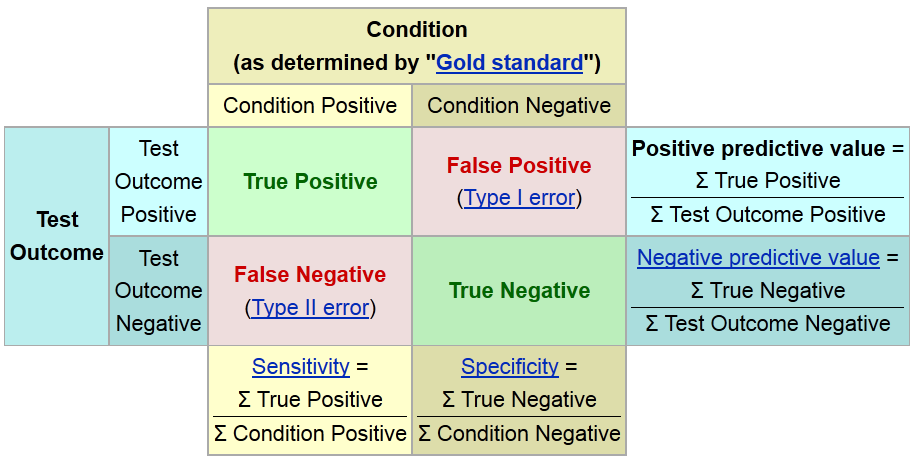
\includegraphics[width=0.75\textwidth]{../Images/Sensitivity_Specificity_Diagram.png}\\
  \caption{Relationship between sensitivity, specificity, positive predictive value and negative predictive value. (From: Wikipedia)}\label{fig:sens_spec_diagram}
\end{figure}

\begin{itemize}
  \item \textbf{Sensitivity} = proportion of positives that are correctly identified by a test = probability of a positive test, given the patient is ill.
  \item \textbf{Specificity} = proportion of negatives that are correctly identified by a test = probability of a negative test, given that patient is well.
  \item \textbf{Positive predictive value} = proportion of patients with positive test results who are correctly diagnosed.
  \item \textbf{Negative predictive value} = proportion of patients with negative test results who are correctly diagnosed.
\end{itemize}

While sensitivity and specificity are independent of prevalence, they do not tell us what portion of patients with abnormal test results are truly abnormal. This information is provided by the positive/negative predictive value. However, as Fig. \ref{fig:prevalence} indicates, these values are affected by the \emph{prevalence} \index{general}{prevalence} of the disease. In other words, we need to know the prevalence of the disease as well as the PPV/NPV of a test to provide a sensible interpretation of the test results.

\begin{figure}[ht]
  \centering
  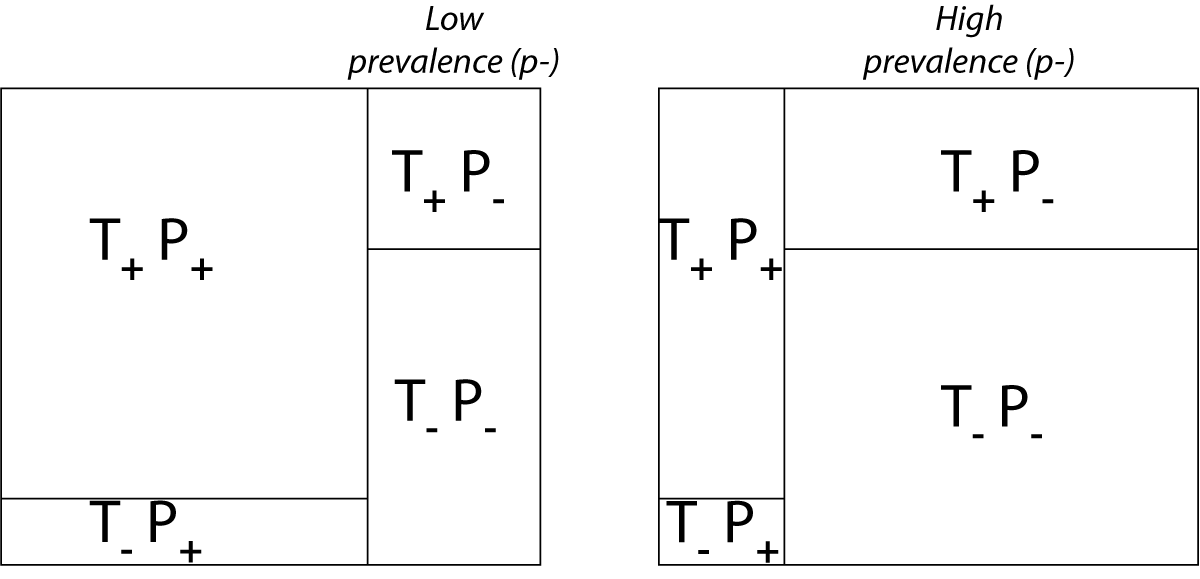
\includegraphics[width=0.75\textwidth]{../Images/Sensitivity_Specificity.png}\\
  \caption{Effect of prevalence on PPV and NPV. "T" stands for "test", and "P" for "patient". (For comparison with below: T+P+ = TP, T-P- = TN, T+P- = FP, and T-P+ = FN)} \label{fig:prevalence}
\end{figure}

Figure \ref{fig:sens_spec_example} gives a worked example:

\begin{figure}[ht]
  \centering
  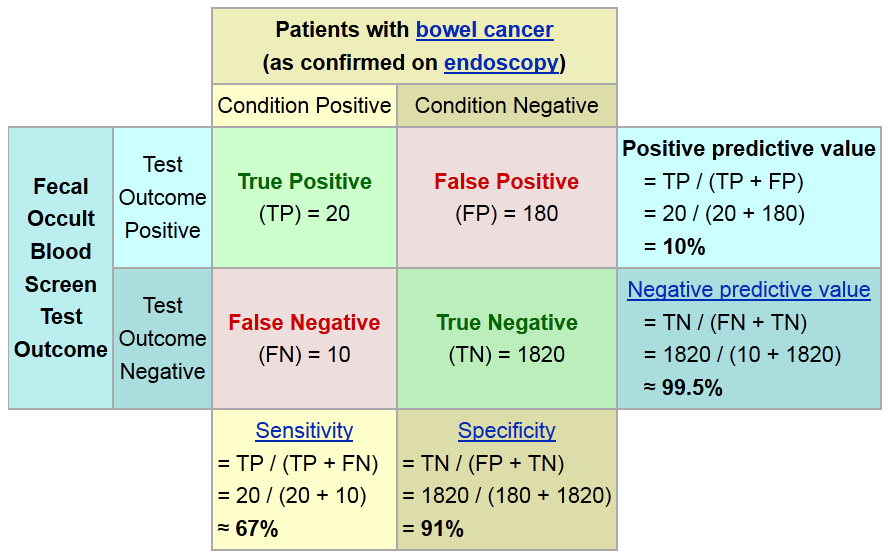
\includegraphics[width=0.75\textwidth]{../Images/Sensitivity_Specificity_Example.png}\\
  \caption{Worked example. (From: Wikipedia)}\label{fig:sens_spec_example}
\end{figure}

\paragraph{Related calculations}

\begin{itemize}
  \item False positive rate ($\alpha$) = type I error = $1 - specificity$ = $\frac{FP}{FP + TN}$ = $\frac{180}{180+1820}$ = 9\%
  \item False negative rate ($\beta$) = type II error = $1 - sensitivity$ = $\frac{FN}{TP + FN}$ = $\frac{10}{20+10}$ = 33\%
  \item Power = sensitivity = $1−\beta$
  \item Likelihood ratio positive = $\frac{sensitivity}{1−specificity}$ = $\frac{66.67\%}{1−91\%}$ = 7.4
  \item Likelihood ratio negative = $\frac{1−sensitivity}{specificity}$ = $\frac{1−66.67\%}{91\%}$ = 0.37
\end{itemize}

Hence with large numbers of false positives and few false negatives, a positive FOB screen test is in itself poor at confirming cancer (PPV = 10\%) and further investigations must be undertaken; it did, however, correctly identify 66.7\% of all cancers (the sensitivity). However as a screening test, a negative result is very good at reassuring that a patient does not have cancer (NPV = 99.5\%) and at this initial screen correctly identifies 91\% of those who do not have cancer (the specificity).

\section{ROC Curve}\index{general}{ROC curve}

Closely related to \emph{Sensitivity} and \emph{Specificity} is the \emph{receiver operating characteristic (ROC)} curve. This is a graph displaying the relationship between the true positive rate (on the vertical axis) and the false positive rate (on the horizontal axis). The technique comes from the field of engineering, where it was developed to find the predictor which best discriminates between two given distributions. In the ROC-curve (Figure \ref{fig:ROC}) this point is given by the value with the largest distance to the diagonal.

\begin{figure}[ht]
  \centering
  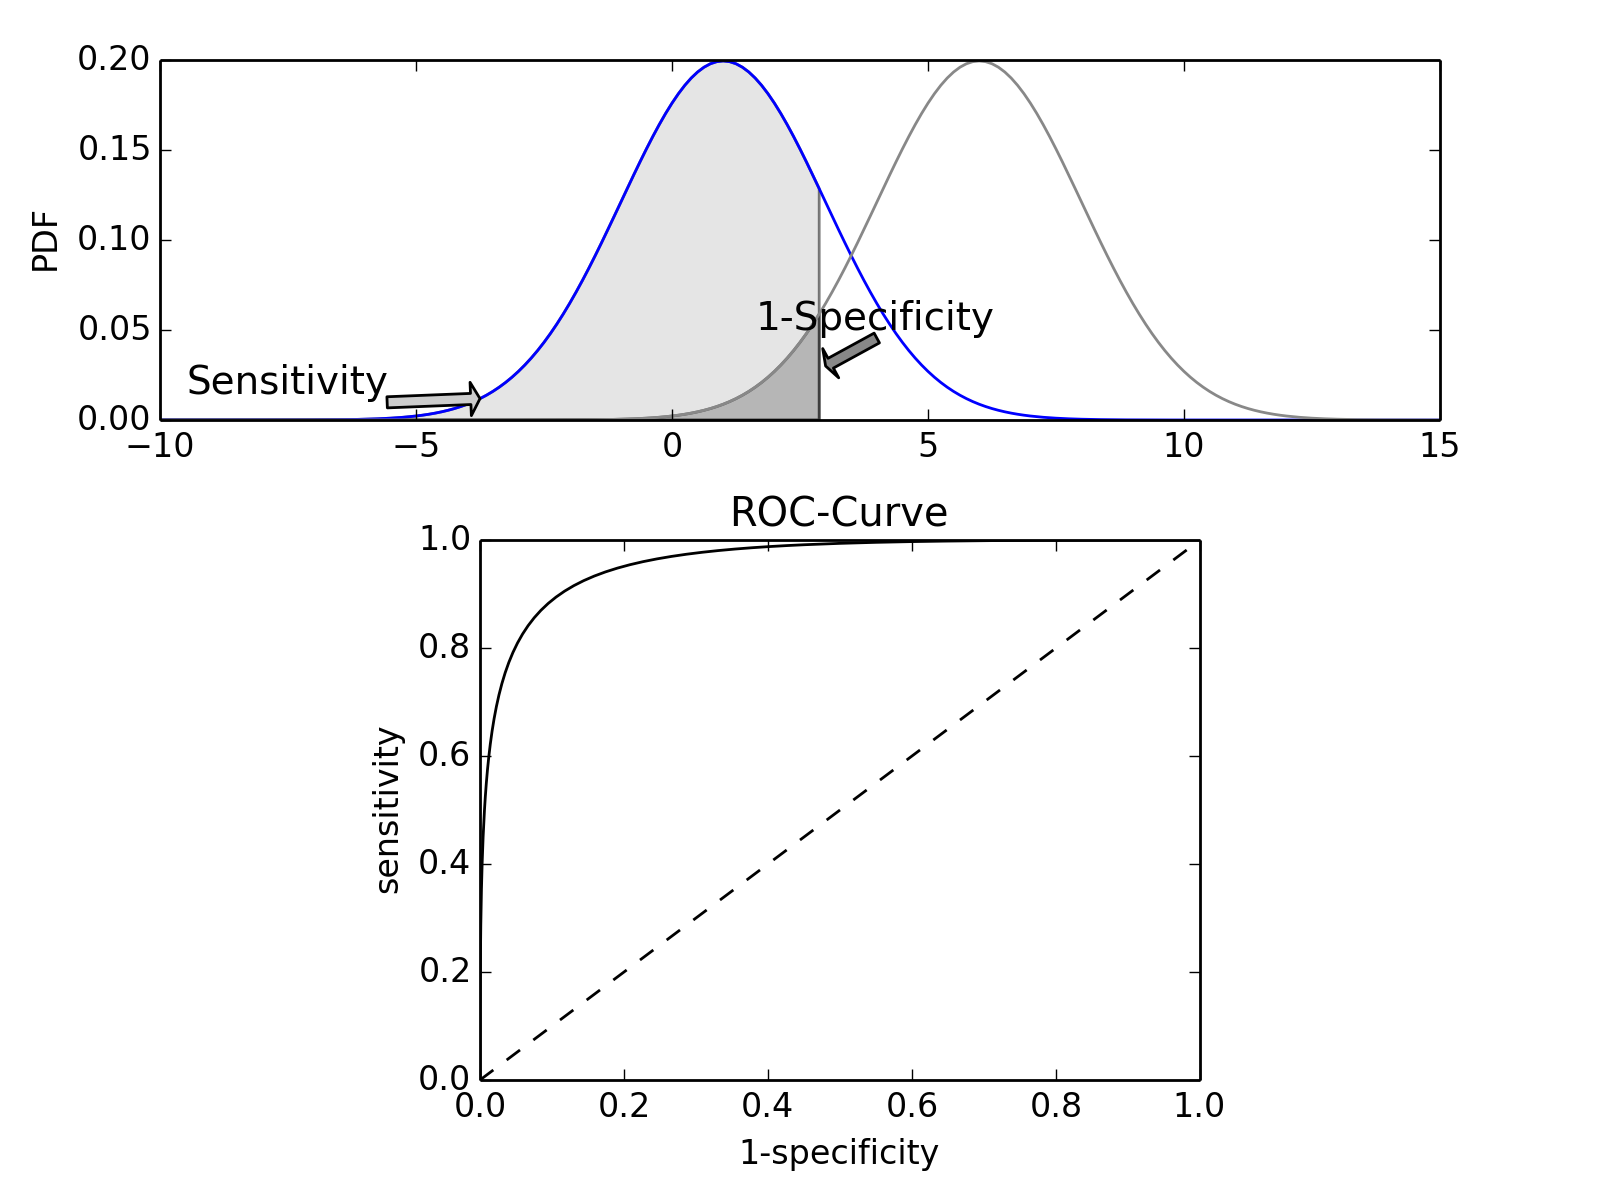
\includegraphics[width=0.75\textwidth]{../Images/ROC.png}\\
  \caption{Top: Probability density functions for two distributions. Bottom: corresponding \emph{ROC-curve}.}\label{fig:ROC}
\end{figure}

\section{Common Statistical Tests for Comparing Groups}

Table \ref{table:tests} gives an overview of the most common statistical tests for different combinations of data.
\begin{table}
  \centering
  \footnotesize{
  \begin{tabular}{ | p{5cm} || p{5cm} | p{5cm} | }
     \hline
     No. of Groups Compared  & \textbf{Independent Samples} & \textbf{Paired Samples} \\ \hline
     \textbf{Groups of Nominal Data} & & \\ \hline
     2 or more & Fisher's exact test or Chi-Square test & McNemar's test \\ \hline
     \textbf{Groups of Ordinal Data} & & \\ \hline
     2 & Mann-Whitney U test & Wilcoxon signed rank test \\ \hline
     3 or more & Kruskal-Wallis test & Friedman test \\ \hline
     \textbf{Groups of Continuous Data} & & \\ \hline
     2 & Student's t-test or Mann-Whitney test & Paired t-test or Wilcoxon signed-rank test \\ \hline
     3 or more & ANOVA or Kruskal-Wallis test & Repeated Measures ANOVA or Friedman test \\ \hline

  \end{tabular}
  }

  \caption{Typical tests for statistical problems.}\label{table:tests}
\end{table}

